\documentclass[a4paper, 12pt]{article}%тип документа

%отступы
\usepackage[left=1.5cm,right=1cm,top=2cm,bottom=3cm,bindingoffset=0cm]{geometry}
\setlength{\parindent}{5ex}

%Русский язык
\usepackage[T2A]{fontenc} %кодировка
\usepackage[utf8]{inputenc} %кодировка исходного кода
\usepackage[english,russian]{babel} %локализация и переносы

%Вставка картинок
\usepackage{graphicx}
\graphicspath{{pictures/}}
\DeclareGraphicsExtensions{.pdf,.png,.jpg,}
\usepackage{wrapfig}

%Графики
\usepackage{pgfplots}
\pgfplotsset{compat=1.9}

%Математика
\usepackage{amsmath, amsfonts, amssymb, amsthm, mathtools}
\usepackage{derivative}

%Таблицы
\usepackage{longtable} 
\usepackage{float}

%Римские цифры
\newcommand{\RomanNumeralCaps}[1]{\uppercase\expandafter{\romannumeral#1}}

\usepackage{multirow}



\begin{document}
	\begin{titlepage}
		\begin{center}
			
			\textsc{Федеральное государственное унитарное предприятие «Центральный научно-исследовательский институт химии и механики» 			\\[5mm]
			}
			
			\vfill
			
			\textbf{Отчет о курсе \\ Введение в специальность
				\\[50mm]
			}
			
		\end{center}
		
		\hfill
		\begin{minipage}{.5\textwidth}
			Выполнил студент:\\[2mm]
			Сериков Василий Романович\\[2mm]
			группа: Б03-102\\[5mm]
			
		\end{minipage}
		\vfill
		\begin{center}
			Москва, 2023 г.
		\end{center}
		
	\end{titlepage}
	
	\newpage
	\setcounter{page}{2}
	
	
	В ходе полугодового курса "Введение в специальность" мы вспомнили курс теоретической механики, а в частности повторили что такое матрицы направляющих косинусов, углы Крылова, углы Эйлера, кинематические и динамические уравнения Эйлера. 
	\begin{figure}[H]
		\centering
		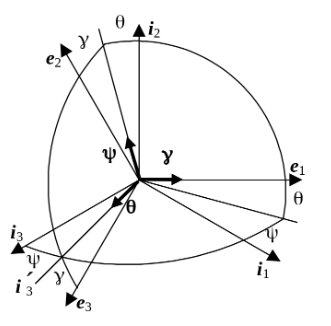
\includegraphics[width=0.3\linewidth]{krilov}
		\caption{Последовательность углов поворота Крылова ($i$ исходный базис, $e$ конечный)}
	\end{figure}
	
	Далее мы познакомились с основными этапами разработки и проектирования систем управления. Разобрали базовые составляющие информационно-измерительного комплекса такие как: магнитный компас, датчик угловой скорости, гироскоп, эхолот, лидар и т.д.	Также описали стадии разработки математической модели подводного, летательного аппарата, записали уравнения динамики.
	
	Разобрались в устройстве и принципе построения бесплатформенных и платформенных инерциальных навигационных систем.
	
	Изучили основные составляющие самолета
	
	\begin{figure}[H]
		\centering
		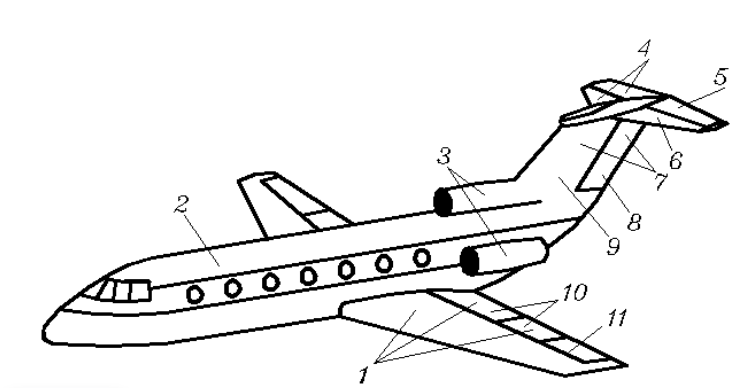
\includegraphics[width=0.6\linewidth]{plane}
		\caption{Самолет и его основные части: 1- крыло; 2- фюзеляж; 3 – силовая установка; 4 – горизонтальное оперение; 5 – руль высоты; 6 – стабилизатор; 7 – вертикальное оперение; 8 – руль направления; 9 –киль; 10 – закрылки; 11 - элерон}
	\end{figure}
	
	
	Изучили различные критерии подобия для летательных аппаратов: 
	
	$$ (\frac{F_{\text{ин}}}{F_{\text{тяж}}})_{\text{нат}} = (\frac{F_{\text{ин}}}{F_{\text{тяж}}})_{\text{мод}} \hspace{4mm} - \text{ По числу Фруда}$$
	
	
	$$ (\frac{E_{\text{кин}}}{E_{\text{внутр}}})_{\text{нат}} = (\frac{E_{\text{кин}}}{E_{\text{внутр}}})_{\text{мод}} \hspace{4mm} - \text{ По сжимаемости }$$
	
	$$ (\frac{VT}{L})_{\text{нат}} = (\frac{VT}{L})_{\text{мод}} \hspace{4mm} - \text{ По числу Струхаля}$$
	
	Также изучили основные уравнения механики и теплообмена:
	
	$$ \pdv{\rho}{t} + \nabla(\rho V)  =  0 \hspace{3mm} - \text{ уравнение неразрывности}$$
	
	$$ \pdv{\rho V}{t} + \nabla \rho V V = \rho f + \nabla \prod_{ij} \hspace{3mm} - \text{ уравнение количества движения} $$
	
	
	\textbf{Заключение: }\\
	
	Подводя итог, можно сказать, что курс "Введение в специальность"  действительно необходим, так как только здесь можно узнать, с чем предстоит иметь дело и что необходимо знать студенту перед устройством на работу. В ходе курса мы обсудили множество устройств и приборов их состав и принцип работы, также описали их работу на математическом языке, опираясь на законы механики. Был изучен большой пласт информации об устройстве летательных и подводных аппаратов. Конечно, хотелось бы больше практики, например работа в MatLab, чтобы пройденная теория не забывалась, а наоборот закреплялась и оставалась в памяти студента и компьютера. 
	
	
	
	
	
	
	
	
	
	
	
	\end{document}